\chapter{Commande temps discret}
Afin d'implémenter la commande, nous allons adapter la commande de façon à ce qu'elle soit exécutable sur le micro-contrôleur. Ensuite, nous évaluerons cette transformation. Nous avons choisi d'implémenter la commande par retour d'état basé observateur car c'est celle que nous avons la plus aboutie compte tenu des spécifications. 
\section{Discrétisation de la commande}
Nous allons à présent transformer la commande en temps continue en une forme qui permet l'implémentation sur un micro-contrôleur. Nous avons choisi de l'implémenter sous la forme d'une équation récurrente. Pour cela, dans un premier temps, nous avons transformer la commande (composée d'un observateur, d'un retour d'état et d'un pré-compensateur) en une forme espace d'états puis nous la discrétiserons. Ensuite, nous allons la transformer en une fonction de transfert pour finalement la transformer en équation récurrente.
	\subsection{Espace d'état à temps discret de la commande}
%		 (observateur + retour état = 2 ft)
%1. obs + re = EE
La commande est de la forme suivante (figure \ref{fig:comTC}) : 
\begin{figure}[!ht]
\centering
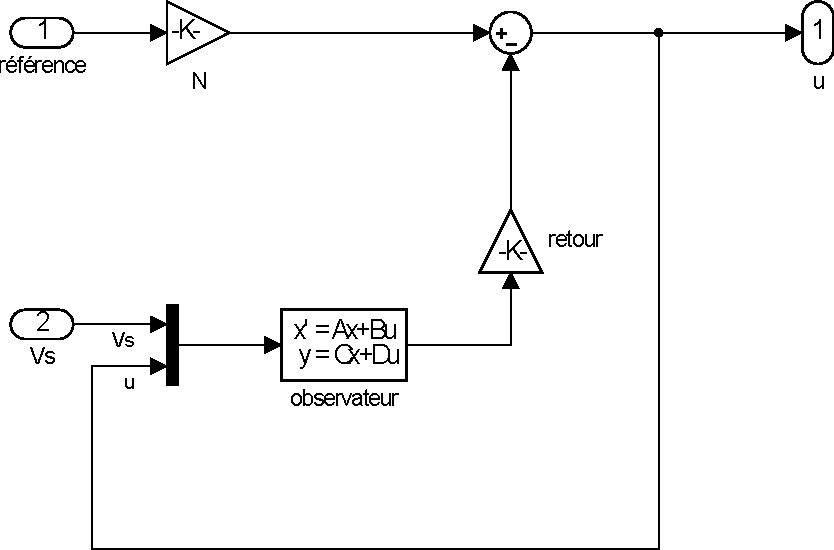
\includegraphics[width=.4\textwidth]{./V/images/Com_asserv.pdf}
\caption{\label{fig:comTC}Schéma de la commande par retour d'état à temps continue.}
\end{figure}


Voici, issue des équations \ref{equ:obs} et \ref{equ:obs2}, l'observateur simplifié (équation \ref{equ:obsSimp}). Nous avons choisi de reconstruire l'observateur avec des valeurs propres désirées accélérée $3$ fois car en simulation, cela réduit l'erreur de gain statique sur le système d'ordre 4 en boucle fermé.
\begin{equation}
\label{equ:obsSimp}
\left\lbrace
\begin{aligned}
&\dot z (t) = Fz(t) + GV_S(t) + Bu(t)\\
&\hat{x}(t) = z(t)
\end{aligned}
\right.
\end{equation}
Ainsi que le retour d'état :
\begin{equation}
u(t) = -K\hat{x}(t) + N V_{ref}(t)
\end{equation}
Nous allons rassembler ces équations afin de créer un nouvel espace d'état:
\begin{equation}
\begin{array}{ll}
&\left\lbrace
\begin{aligned}
&\dot z (t) = Fz(t) + GV_S(t) + Bu(t)\\
&u(t) = -Kz(t) + N V_{ref}(t)
\end{aligned}
\right.
\Leftrightarrow
\left\lbrace
\begin{aligned}
&\dot z (t) = (F-KB)z(t) + GV_S(t) + BN V_{ref}(t)\\
&u(t) = -Kz(t) + N V_{ref}(t)
\end{aligned}
\right.\\
&\\

\Leftrightarrow&
\left\lbrace
\begin{aligned}
&\dot z (t) = (F-KB)z(t) + 
\begin{bmatrix} BN &  G  \end{bmatrix}  
\begin{bmatrix}  V_{ref}(t) \\ V_S(t) \end{bmatrix}  
\\
&u(t) = -Kz(t) + 
\begin{bmatrix} N &  0 \end{bmatrix}  
\begin{bmatrix} V_{ref}(t) \\ V_S(t) \end{bmatrix}  
\end{aligned}
\right.
\end{array}
\end{equation}
%2. EE(z)
Maintenant que nous avons exprimer la commande sous la forme d'un espace d'état, avec pour entrées $V_{ref}(t)$ la consigne et $V_S(t)$, la sortie de position mesurée, nous pouvons discrétiser la commande. Nous avons choisis de discrétiser la commande grâce à matlab, avec l'option \emph{zoh} afin de discrétiser la commande avec un bloqueur d'ordre 0 : \begin{equation}
 B_O(p)=\frac{1 - e^{-pT_e}}{p}
 \end{equation}
 Où $Te=0.052$ secondes, c'est a dire $5.2$ fois la fréquence maximale propre au moteur (voir chapitre \ref{chap:implem}.
Cela donne la commande à temps discret suivante :
\begin{equation}
\label{equ:EEcomTD}
\begin{array}{rl}
& \left\lbrace
\begin{array}{rclcl}
z(z-1) 	&=& A z(z) &+& B \begin{bmatrix} V_{ref}(t) \\ V_S(t)  \end{bmatrix}  \\
u(z)  	&=& C z(z) &+& D \begin{bmatrix} V_{ref}(t) \\ V_S(t)  \end{bmatrix}  
\end{array}
\right.\\
&\\
\Leftrightarrow &
\left\lbrace
\begin{array}{rclcclc}
z(z-1) 	&=& 
\begin{bmatrix}
-23.05   	&   1\\
-88.94    	&  	-9
\end{bmatrix} &z(z) 
&+& \begin{bmatrix}
0  		&	20.74\\
85.71 	&	80.05
\end{bmatrix} 
&\begin{bmatrix} V_{ref}(t) \\ V_S(t)  \end{bmatrix}  \\
u(z)  	&=& \begin{bmatrix}
0 		&	 -0.08899
\end{bmatrix} &z(z) &+& \begin{bmatrix}
1.511  	&    0
\end{bmatrix} 
&\begin{bmatrix} V_{ref}(t) \\ V_S(t)  \end{bmatrix}  
\end{array}
\right.
\end{array}
\end{equation}



 

 


	\subsection{Équation récurrente}
%1. EE 		= 2*tf(z)
	Nous allons maintenant transformer l'espace d'état de l'équation \ref{equ:EEcomTD} en fonctions de transferts, à l'aide de matlab :
\begin{eqnarray}
\frac{u(z)}{V_{ref}(z)}	&=&	\frac{1.511 z^2 - 1.551 z + 0.3757}{    z^2 - 0.8231 z +  0.1889}\\
\frac{u(z)}{V_s(z)} &=& \frac{-0.1581 z + 0.1581}{    z^2 - 0.8231 z +  0.1889}
\end{eqnarray}

%2. 2*tf(z) = 1*tf(z^-1)

Afin d'avoir une commande causale, nous avons passer les fonctions de transferts en $z^{-1}$ :
\begin{eqnarray}
\label{equ:ftTD1}\frac{u(z^{-1})}{V_{ref}(z^{-1})} &=& \frac{1.511 - 1.551 z^{-1} + 0.3757 z^{-2}}{    1 - 0.8231 z^{-1} +  0.1889z^{-2}}\\
\label{equ:ftTD2}\frac{u(z^{-1})}{V_s(z^{-1})}	&=&	\frac{-0.1581 z^{-1} + 0.1581z^{-2}}{    1 - 0.8231 z^{-1} +  0.1889z^{-2}}
\end{eqnarray}
Nous avons ensuite, à partir des équations \ref{equ:ftTD1} et  \ref{equ:ftTD2}, créer une seule équation :
\begin{equation}
\label{equ:eqTDz-}
\begin{array}{lcl}
u(z^{-1})(1 - 0.8231 z^{-1} +  0.1889 z^{-2}) &=& (1.511 - 1.551 z^{-1} + 0.3757 z^{-2})  V_{ref}(z^{-1}) \\
&&+ (-0.1581 z^{-1} + 0.1581z^{-2})V_{s}(z^{-1})
\end{array}
\end{equation}
Nous avons maintenant une seule équation pour représenter la commande à temps discret.%
%3. tf(z^-1)= ER(z^-1)
Il faut maintenant la transformée en équation récurrente, pour cela nous allons utiliser la propriété suivante :
\begin{equation}
f(z)z^n = f_{k+n}
\end{equation}
Cela donne, une fois réorganiser de façon à isoler la sortie $u_k$ et à partir de l'équation \ref{equ:eqTDz-} :
\begin{equation}
\begin{array}{lcl}
u_k &=&  0.8231 u_{k-1} - 0.1889  u_{k-2} \\
&& + 1.511 Vr_k - 1.551 Vr_{k-1}  + 0.3757 Vr_{k-2}\\
&& - 0.1581 Vs_{k-1} + 0.1581 Vs_{k-2}  \\
\end{array}
\end{equation}
Où, par soucis de lisibilité, $Vs = V_s$ et $Vr = V_{ref}$.
Le coût temporel de ce calcul est au minimum de $7*400ns = 2.8 ms$.




\section{Test de la commande en simulation}
Afin de vérifier que la commande est bien fonctionnelle à temps discret, nous avons créer un modèle Simulink qui test la commande sous la forme d'une équation récurrente sur les modèles d'ordre 2, 3 et 4. 
Voici, figure \ref{fig:simuER}, les réponses de ces asservissements à un signal rectangulaire d'amplitude 3 Volts.
\begin{figure}[!ht]
\centering
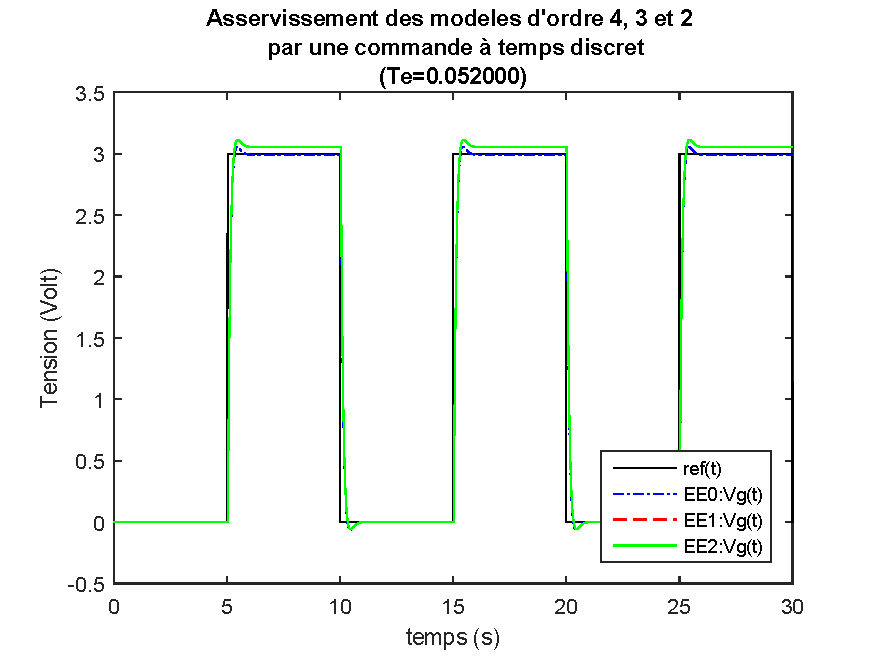
\includegraphics[width=.5\textwidth]{./V/images/AsserTDEqRec.pdf}
\caption{\label{fig:simuER}Réponse des systèmes en boucle fermée asservis par équations récurrentes.}
\end{figure}

Nous pouvons voir que l'erreur statique et le temps de réponse sont important sur l'ordre 2 mais réduisent sur les ordres 3 et 4. 

Maintenant que nous avons une équation implémentable sur micro-contrôleur, il faut créer un code le permettant, à partir de celui fourni.
